\subsubsection{x86: 3 argomenti}

\myparagraph{MSVC}

Quando compiliamo l'esempio con MSVC 2010 Express otteniamo:

\begin{lstlisting}
$SG3830	DB	'a=%d; b=%d; c=%d', 00H

...

	push	3
	push	2
	push	1
	push	OFFSET $SG3830
	call	_printf
	add	esp, 16					; 00000010H
\end{lstlisting}

Notiamo che gli argomenti di \printf sono messi sullo stack in ordine inverso. Il primo argomento e' quello messo per ultimo.

A proposito, le variabili di tipo \Tint in ambienti a 32-bit hanno dimensione pari a 32-bit, ovvero 4 byte.

Abbiamo 4 argomenti, quindi $4*4 = 16$~---essi occupano esattamente 16 bytes nello stack: un puntatore a 32-bit alla stringa,  e 3 numeri di tipo \Tint.

\myindex{x86!\Instructions!ADD}
\myindex{x86!\Registers!ESP}
\myindex{cdecl}
Quando lo \gls{stack pointer} (registro \ESP) viene ripristinato dall'istruzione \INS{ADD ESP, X}
dopo una chiamata a funzione, in molti casi il numero di argomenti della fuznione puo' essere dedotto semplicemente dividendo X per 4.

Questa caratteristca  e' propria solo della calling convention \IT{cdecl} e in ambienti a 32-bit..

Si veda anche la sezione sulle calling conventions ~(\myref{sec:callingconventions}).

In certi casi in qui diverse funzioni ritornano una dopo l'altra, il compilatore potrebbe accorpare piu' istruzioni \q{ADD ESP, X} 
dopo l'ultima chiamata, emettendo una sola istruzione:

\begin{lstlisting}
push a1
push a2
call ...
...
push a1
call ...
...
push a1
push a2
push a3
call ...
add esp, 24
\end{lstlisting}

Ecco un esempio reale:

% TODO translate to Italian
\lstinputlisting[caption=x86]{patterns/03_printf/x86/add_example_EN.lst}

\clearpage
\myparagraph{MSVC and \olly}
\myindex{\olly}

Proviamo ora ad esaminare l'esempio con \olly, uno dei piu' diffusi debugger win32 user-land.
Possiamo compilarlo in MSVC 2012 con l'opzione \GTT{/MD}, che indica al compilatore di linkare con \GTT{MSVCR*.DLL},
in maniera tale da poter vedere in modo chiaro, nel debugger, le funzioni importate.

Carichiamo quindi l'eseguibile in \olly.
Il primo breakpoint avviene in \GTT{ntdll.dll}, premiamo F9 (run) per continuare l'esecuzione. 
Il secondo breakpoint e' nel codice \ac{CRT}.
Ora dobbiamo trovare la funzione \main.

Per farlo scorriamo il codice verso l'alto (MSVC alloca la funzione \main proprio all'inizio della sezione code): 
\begin{figure}[H]
\centering
\myincludegraphics{patterns/03_printf/x86/olly3_1.png}
\caption{\olly: the very start of the \main function}
\label{fig:printf3_olly_1}
\end{figure}

Clickiamo sull'istruzione \INS{PUSH EBP}, premiamo F2 (set breakpoint) and quindi F9 (run).
Queste azioni ci consentono di saltare tutta la parte legata al codice \ac{CRT}, in quanto per il momento non ci interessa.

\clearpage
Premiamo F8 (\stepover) 6 volte, ovverso saltiamo (avanziamo di) 6 istruzioni:

\begin{figure}[H]
\centering
\myincludegraphics{patterns/03_printf/x86/olly3_2.png}
\caption{\olly: before \printf execution}
\label{fig:printf3_olly_2}
\end{figure}

Adesso il \ac{PC} punta all'istruzione \INS{CALL printf}.
\olly, come altri debugger, evidenzia il valore dei registri che sono stati modificati.
Quindi ogni volta che si preme F8, \EIP cambia ed il suo valore e' mostrato in rosso.
Anche \ESP cambia, poiche' i valori degli argomenti vengono messi sullo stack.

Dove sono i valori messi nello stack?
Diamo un'occhiata alla finestra del debugger in basso a destra:

\begin{figure}[H]
\centering
\ifdefined\ebook
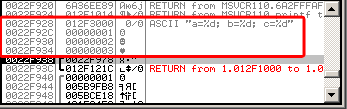
\includegraphics[width=\textwidth]{patterns/03_printf/x86/olly3_stack.png}
\else
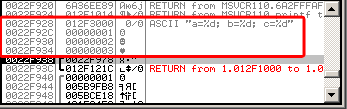
\includegraphics[width=0.5\textwidth]{patterns/03_printf/x86/olly3_stack.png}
\fi

\caption{\olly: stato dello stack dopo il push dei valori degli argomenti (il rettangolo rosso e' stato aggiunto dall'autore per evidenziare la finestra)}
\end{figure}

Notiamo 3 colonne: indirizzo nello stack, valore nello stack ed alcuni commenti aggiuntivi di \olly. 
\olly riconosce le stringhe \printf{}-like , e riporta quindi la stringa insieme ai 3 valori \IT{associati}.

Facendo click destro sulla formato string, quindi click su \q{Follow in dump},
e' possibile vedere la format string nella finestra del debugger in basso a sinistra, che mostra una zona di memoria.
I valori mostrati possono anche essere modificati.
E' ad esempio possibile cambiare la format string, che renderebbe diverso il risultato dell'esempio.
Non e' molto utile in questo particolare caso, ma puo' comunque essere un esercizio utile per iniziare a prendere dimestichezza con lo strumento.

\clearpage
Premiamo F8 (\stepover).

Il seguente output viene riportato in console:

\lstinputlisting{patterns/03_printf/x86/console.txt}

Vediamo come sono cambiati i registri e lo stack:

\begin{figure}[H]
\centering
\myincludegraphics{patterns/03_printf/x86/olly3_3.png}
\caption{\olly dopo dell'esecuzione di \printf{}}
\label{fig:printf3_olly_3}
\end{figure}

Il registro \EAX adesso contiene \GTT{0xD} (13).
Questo valore e' corretto, poiche' \printf restituisce il numero di caratteri stampati. 
Il valore di \EIP e' cambiato: adesso contiene infatti l'indirizzo dell'istruzione che viene dopo \INS{CALL printf}.
Anche i valori \ECX e \EDX sono cambiati.
Apparentemente, i meccanismi interni alla funzione \printf hanno usato quei registri durante l'esecuzione di printf per le sue necessita'.

Un fatto molto importante e' che ne' il valore di ESP ne' lo stack sono stati modificati!
Vediamo chiaramente che la format string ed i suoi 3 valori si trovano ancora li'.
Questo e; infatti il comportamento della calling convention \IT{cdecl}: il \gls{callee} (la funzione chiamata) non ripristina
\ESP al suo valore precedente. Farlo e' una responsabilita' del The \gls{caller} (chiamante).

\clearpage
Premiamo F8 nuovamente per eseguire l'istruzione \INS{ADD ESP, 10}:

\begin{figure}[H]
\centering
\myincludegraphics{patterns/03_printf/x86/olly3_4.png}
\caption{\olly: after \INS{ADD ESP, 10} instruction execution}
\label{fig:printf3_olly_4}
\end{figure}

\ESP e' cambiato, ma i valori si trovano ancora sullo stack!
Ovviamente si: non c'e' necessita' di azzerare i valori o effettuare altre simili operazioni di "pulizia".
Qualunque cosa si trovi sopra lo stack pointer (\ac{SP}) e' \IT{noise} o \IT{\garbage{}} e non ha alcun significato.
Pulire i valori non utilizzati nello stack sarebbe una perdita di tempo inutile, e non vi e' alcuna necessita' di farlo.

\myparagraph{GCC}

Compiliamo adesso lo stesso programma su Linux usando GCC 4.4.1, e diamo un'occhiata al risultato con \IDA:

\begin{lstlisting}
main            proc near

var_10          = dword ptr -10h
var_C           = dword ptr -0Ch
var_8           = dword ptr -8
var_4           = dword ptr -4

                push    ebp
                mov     ebp, esp
                and     esp, 0FFFFFFF0h
                sub     esp, 10h
                mov     eax, offset aADBDCD ; "a=%d; b=%d; c=%d"
                mov     [esp+10h+var_4], 3
                mov     [esp+10h+var_8], 2
                mov     [esp+10h+var_C], 1
                mov     [esp+10h+var_10], eax
                call    _printf
                mov     eax, 0
                leave
                retn
main            endp
\end{lstlisting}

Si nota che la differenza tra il codice prodotto da MSVC e GCC risiede soltanto nel modo in cui gli argomenti sono memorizzati sullo stack.
In questo caso GCC lavora diversamente con lo stack senza l'uso di \PUSH/\POP.

\myparagraph{GCC e GDB}
\myindex{GDB}

Proviamo l'esempio anche con \ac{GDB} su Linux.

L'opzione \GTT{-g} indica al comiplatore di includere le informazioni di debug nel file eseguibile.

\begin{lstlisting}
$ gcc 1.c -g -o 1
\end{lstlisting}

\begin{lstlisting}
$ gdb 1
GNU gdb (GDB) 7.6.1-ubuntu
Copyright (C) 2013 Free Software Foundation, Inc.
License GPLv3+: GNU GPL version 3 or later <http://gnu.org/licenses/gpl.html>
This is free software: you are free to change and redistribute it.
There is NO WARRANTY, to the extent permitted by law.  Type "show copying"
and "show warranty" for details.
This GDB was configured as "i686-linux-gnu".
For bug reporting instructions, please see:
<http://www.gnu.org/software/gdb/bugs/>...
Reading symbols from /home/dennis/polygon/1...done.
\end{lstlisting}

\begin{lstlisting}[caption=impostiamo un breakpoint su \printf]
(gdb) b printf
Breakpoint 1 at 0x80482f0
\end{lstlisting}

Avviamolo.
Non abbiamo il sorgente della funzione \printf qui, quindi \ac{GDB} non puo' mostrarlo, anche se potrebbe.

\begin{lstlisting}
(gdb) run
Starting program: /home/dennis/polygon/1 

Breakpoint 1, __printf (format=0x80484f0 "a=%d; b=%d; c=%d") at printf.c:29
29	printf.c: No such file or directory.
\end{lstlisting}

Stampiamo 10 elementi dello stack elements. La colonna piu' a sinistra contiene l'indirizzo nello stack.

\begin{lstlisting}
(gdb) x/10w $esp
0xbffff11c:	0x0804844a	0x080484f0	0x00000001	0x00000002
0xbffff12c:	0x00000003	0x08048460	0x00000000	0x00000000
0xbffff13c:	0xb7e29905	0x00000001
\end{lstlisting}

Il primo elemento e' il \ac{RA} (\GTT{0x0804844a}).
Possiamo verificarlo disassemblando la memoria a questo indirizzo:

\begin{lstlisting}[label=NOP_as_XCHG_example]
(gdb) x/5i 0x0804844a
   0x804844a <main+45>:	mov    $0x0,%eax
   0x804844f <main+50>:	leave  
   0x8048450 <main+51>:	ret    
   0x8048451:	xchg   %ax,%ax
   0x8048453:	xchg   %ax,%ax
\end{lstlisting}

Le due istruzioni \INS{XCHG} sono istruzioni \q{inutili} (idle), analoghe a \ac{NOP}.

Il secondo elemento (\GTT{0x080484f0}) e' l'indirizzo della format string:

\begin{lstlisting}
(gdb) x/s 0x080484f0
0x80484f0:	"a=%d; b=%d; c=%d"
\end{lstlisting}

I successivi 3 elementi (1, 2, 3) sono gli argomenti di \printf.
Il resto degli elementi potrebbe essere \q{immondizia} nello stack, oppure valori provenienti da altre funzioni, come le loro variabili locali, etc.
Per il momento li possiamo ignorare.

Eseguiamo il comando \q{finish}. 
Questo comando dice a GDB di \q{eseguire tutte le istruzioni fino alla fine della funzione}.
In questo caso: esegui fino alla fine di \printf.

\begin{lstlisting}
(gdb) finish
Run till exit from #0  __printf (format=0x80484f0 "a=%d; b=%d; c=%d") at printf.c:29
main () at 1.c:6
6		return 0;
Value returned is $2 = 13
\end{lstlisting}

\ac{GDB} mostr il risultato di \printf restituito in \EAX (13).
Questo e' il numero di caratteri stampati, proprio come nell'esempio in \olly.

Vediamo anche \q{return 0;} e l'informazione che questa espressione si trova nel file \GTT{1.c} a riga 6.
Infatti il file \GTT{1.c} si trova nella directory corrente, e \ac{GDB} trova la stringa li'.
Come fa \ac{GDB} a sapere quale riga del codice C viene eseguita?
Cio' e' dovuto al fatto che il compilatore, quando genera le informazioni di debug, salva anche una tabella di relazioni tra le righe del
codice sorgente e gli indirizzi delle istruzioni.
Dopotutto GDB e' un \q{source-level debugger}.

Esaminiamo i registri.
13 in \EAX:

\begin{lstlisting}
(gdb) info registers
eax            0xd	13
ecx            0x0	0
edx            0x0	0
ebx            0xb7fc0000	-1208221696
esp            0xbffff120	0xbffff120
ebp            0xbffff138	0xbffff138
esi            0x0	0
edi            0x0	0
eip            0x804844a	0x804844a <main+45>
...
\end{lstlisting}

Disassembliamo le istruzioni correnti.
La freccia punta all'a prossima istruzione da eseguire.

\begin{lstlisting}
(gdb) disas
Dump of assembler code for function main:
   0x0804841d <+0>:	push   %ebp
   0x0804841e <+1>:	mov    %esp,%ebp
   0x08048420 <+3>:	and    $0xfffffff0,%esp
   0x08048423 <+6>:	sub    $0x10,%esp
   0x08048426 <+9>:	movl   $0x3,0xc(%esp)
   0x0804842e <+17>:	movl   $0x2,0x8(%esp)
   0x08048436 <+25>:	movl   $0x1,0x4(%esp)
   0x0804843e <+33>:	movl   $0x80484f0,(%esp)
   0x08048445 <+40>:	call   0x80482f0 <printf@plt>
=> 0x0804844a <+45>:	mov    $0x0,%eax
   0x0804844f <+50>:	leave  
   0x08048450 <+51>:	ret    
End of assembler dump.
\end{lstlisting}

\ac{GDB} usa la sintassi AT\&T di default.
Ma e' anche possibile passare alla sintassi Intel:

\begin{lstlisting}
(gdb) set disassembly-flavor intel
(gdb) disas
Dump of assembler code for function main:
   0x0804841d <+0>:	push   ebp
   0x0804841e <+1>:	mov    ebp,esp
   0x08048420 <+3>:	and    esp,0xfffffff0
   0x08048423 <+6>:	sub    esp,0x10
   0x08048426 <+9>:	mov    DWORD PTR [esp+0xc],0x3
   0x0804842e <+17>:	mov    DWORD PTR [esp+0x8],0x2
   0x08048436 <+25>:	mov    DWORD PTR [esp+0x4],0x1
   0x0804843e <+33>:	mov    DWORD PTR [esp],0x80484f0
   0x08048445 <+40>:	call   0x80482f0 <printf@plt>
=> 0x0804844a <+45>:	mov    eax,0x0
   0x0804844f <+50>:	leave  
   0x08048450 <+51>:	ret    
End of assembler dump.
\end{lstlisting}

Eseguiamo la prossima istruzione.
\ac{GDB} mostra la parentesi graffa chiusa, che sta a significare la fine del blocco di codice.

\begin{lstlisting}
(gdb) step
7	};
\end{lstlisting}

Esaminiamo i registri dopo l'esecuzione dell'istruzione \INS{MOV EAX, 0}.
\EAX e' zero.

\begin{lstlisting}
(gdb) info registers
eax            0x0	0
ecx            0x0	0
edx            0x0	0
ebx            0xb7fc0000	-1208221696
esp            0xbffff120	0xbffff120
ebp            0xbffff138	0xbffff138
esi            0x0	0
edi            0x0	0
eip            0x804844f	0x804844f <main+50>
...
\end{lstlisting}
